\documentclass[10pt,a4paper]{article}
\usepackage{graphicx}
\usepackage{biblatex}
\usepackage{parskip}
\usepackage{listings}
\usepackage{caption}
\usepackage{subcaption}
\usepackage{amsmath}
\usepackage[most]{tcolorbox}
\usepackage{xcolor}

\lstset{basicstyle=\ttfamily, breaklines = true, tabsize=2}
\graphicspath{ {./Images/} }
\setlength{\parskip}{1em}
\begin{document}
%%%%%%%%%%%%%%%%%%%%%%%%%%%%%%%%%%%%%%%%%%%%%%%%%%%%%%%%%%%%%%%%%%%%%%%%%%%%%%%%%%%%%%%%%%%%%%%%%%%%%%%%%%
\definecolor{Code}{rgb}{0,0,0} 
\definecolor{Decorators}{rgb}{0.5,0.5,0.5} 
\definecolor{Numbers}{rgb}{0.5,0,0} 
\definecolor{MatchingBrackets}{rgb}{0.25,0.5,0.5} 
\definecolor{Keywords}{rgb}{0,0,1} 
\definecolor{self}{rgb}{0,0,0} 
\definecolor{Strings}{rgb}{0,0.63,0} 
\definecolor{Comments}{rgb}{0,0.63,1} 
\definecolor{Backquotes}{rgb}{0,0,0} 
\definecolor{Classname}{rgb}{0,0,0} 
\definecolor{FunctionName}{rgb}{0,0,0} 
\definecolor{Operators}{rgb}{0,0,0} 
\definecolor{Background}{rgb}{0.98,0.98,0.98}

\lstdefinelanguage{Python}{ 
numbers=left, 
numberstyle=\footnotesize, 
numbersep=1em, 
xleftmargin=1em, 
framextopmargin=2em, 
framexbottommargin=2em, 
showspaces=false, 
showtabs=false, 
showstringspaces=false, 
frame=l, 
tabsize=4, 
% Basic 
basicstyle=\ttfamily,
backgroundcolor=\color{Background}, 
% Comments 
commentstyle=\color{Comments}\slshape, 
% Strings 
stringstyle=\color{Strings}, 
morecomment=[s][\color{Strings}]{"""}{"""}, 
morecomment=[s][\color{Strings}]{'''}{'''}, 
% keywords 
morekeywords={import,from,class,def,for,while,if,is,in,elif,else,not,and,or,print,break,continue,return,True,False,None,access,as,,del,except,exec,finally,global,import,lambda,pass,print,raise,try,assert}, 
keywordstyle={\color{Keywords}\bfseries}, 
% additional keywords 
morekeywords={[2]@invariant,pylab,numpy,np,scipy}, 
keywordstyle={[2]\color{Decorators}\slshape}, 
emph={self}, 
emphstyle={\color{self}\slshape}, 
% 
} 
        
%%%%%%%%%%%%%%%%%%%%%%%%%%%%%%%%%%%%%%%%%%%%%%%%%%%%%%%%%%%%%%%%%%%%%%%%%%%%%%%%%%%%%%%%%%%%%%%%%%%%%%%%%%
\begin{titlepage}
	\centering
	{\scshape\LARGE Imperial College London \par}
	\vspace{1cm}
	{\scshape\Large Mathematics: Year 2\par}
	\vspace{1.5cm}
	{\huge\bfseries Numerical Analysis\par}
	\vspace{2cm}
	{\Large\ Xin Wang }
	\vfill
	{\large \today\par}
\end{titlepage}

%%%%%%%%%%%%%%%%%%%%%%%%%%%%%%%%%%%%%%%%%%%%%%%%%%%%%%%%%%%%%%%%%%%%%%%%%%%%%%%%%%%%%%%%%%%%%%%%%%%%%%%%%%

\begin{abstract}
    Equations that represent mathematical models in engineering involve derivatives (\textbf{differential
    equations}) and integrals (\textbf{integral equations} or \textbf{integro-differential
    equations}) of the variables associated with the models.\par 
    
    While some differential equations can be solved, the vast majority cannot be solved, only
    approximations can be made. There are many techniques for analyzing the various differential 
    equations. Many differential equations cannot be solved exactly thus will require numerical 
    solutions to approximate the equations. Each numerical solution technique has varying levels of 
    error in approximation under different circumstances so choosing the right one is important.
\end{abstract}

%%%%%%%%%%%%%%%%%%%%%%%%%%%%%%%%%%%%%%%%%%%%%%%%%%%%%%%%%%%%%%%%%%%%%%%%%%%%%%%%%%%%%%%%%%%%%%%%%%%%%%%%%%

\tableofcontents
\pagebreak
\lstlistoflistings
\pagebreak

%%%%%%%%%%%%%%%%%%%%%%%%%%%%%%%%%%%%%%%%%%%%%%%%%%%%%%%%%%%%%%%%%%%%%%%%%%%%%%%%%%%%%%%%%%%%%%%%%%%%%%%%%%
\section{Arithmetic and error analysis}
%%%%%%%%%%%%%%%%%%%%%%%%%%%%%%%%%%%%%%%%%%%%%%%%%%%%%%%%%%%%%%%%%%%%%%%%%%%%%%%%%%%%%%%%%%%%%%%%%%%%%%%%%%
\subsection{Exponential notation}

Real numbers can have a finite or infinite number of digits. In order to work with real numbers, the
numbers have to be approximated using a finite number of digits - usually in a standard way to allow
efficient recognition of its magnitude. This is the reason why \textbf{scientific notation} is used,
leading to the establishment of IEEE-754 for use in computing.

Due to the fundamental design of computers and the finite number of digits used in calculations,
there will always be an inherent difference between the calculated value and the real value.

%%%%%%%%%%%%%%%%%%%%%%%%%%%%%%%%%%%%%%%%%%%%%%%%%%%%%%%%%%%%%%%%%%%%%%%%%%%%%%%%%%%%%%%%%%%%%%%%%%%%%%%%%%
\subsection{Error analysis}

Any approximation of a function necessarily allows a possibility of deviation from the correct value of the function.

\begin{tcolorbox}[breakable,colback=white]
    \textbf{Error}: The term used to denote the amount by which an approximation fails to equal the exact solution.
\end{tcolorbox}

There are various kinds of errors:
\begin{itemize}
    \item \textbf{Absolute error}: Value when $\hat{x}$ used instead of $x$
    $$
        |\hat{x} - x|
    $$
    \item \textbf{Relative error}: Value when $\hat{x}$ used instead of $x$
    $$
        \frac{|\hat{x} - x|}{|x|}
    $$
\end{itemize}

There are multiple possible sources of error:
\begin{itemize}
    \item \textbf{Measurement error}: Self-explanatory.
    \item \textbf{Truncation error}: Occurs when a calculated number has more digits than available and some of them must be “forgotten”.
    \item \textbf{Rounding error}: Occurs when a number is rounded to a specified precision.
    \item \textbf{Loss of significance} or \textbf{Cancellation error}: Occurs when an operation on
    two numbers increases relative error substantially more than the absolute  error.   
\end{itemize}

\pagebreak
%%%%%%%%%%%%%%%%%%%%%%%%%%%%%%%%%%%%%%%%%%%%%%%%%%%%%%%%%%%%%%%%%%%%%%%%%%%%%%%%%%%%%%%%%%%%%%%%%%%%%%%%%%
\section{Ordinary Differential Equations (ODE)}

The main application of numerical methods is for integrating differential equations (which why it is
called Numerical Methods - for “solving them numerically”).

%%%%%%%%%%%%%%%%%%%%%%%%%%%%%%%%%%%%%%%%%%%%%%%%%%%%%%%%%%%%%%%%%%%%%%%%%%%%%%%%%%%%%%%%%%%%%%%%%%%%%%%%%%
\subsection{Basics of an ODE}

\begin{tcolorbox}[breakable,colback=white]
\textbf{Ordinary Differential Equation} (ODE): An equality $A=B$ in which the only unknown $(y)$ is
a function of one variable whose derivative of some order appears explicitly $(x)$ or $(t)$.
\end{tcolorbox}

The \textit{ordinary} in ODE is the condition on the unknown being a function of a \textbf{single
variable} i.e. there are no partial derivatives. 

A typical ODE has a general form of:
$$
y^{\prime}=f(x,y)
$$
and \textbf{may} have an exact (analytical) solution. However, more complicated functions $f(x,y)$ make
it difficult and unsustainable to find. Numerical methods are faster and more efficient. These
methods also apply to higher order ODEs such as 2nd Order Differential Equations.

%%%%%%%%%%%%%%%%%%%%%%%%%%%%%%%%%%%%%%%%%%%%%%%%%%%%%%%%%%%%%%%%%%%%%%%%%%%%%%%%%%%%%%%%%%%%%%%%%%%%%%%%%%
\subsection{Euler's Method}

Euler's method is a \textit{first-order} numerical method for solving ODEs with a given initial
value. It is the most basic explicit method for numerical integration of ordinary differential
equations and is the simplest Runge–Kutta method. 

The Euler method is a first-order method, which means that the local error (error per step) is
proportional to the square of the step size, and the global error (error at a given time) is
proportional to the step size. It forms the basis for more complex methods such as the
"predictor-corrector method". 
 
Euler's method proposes a method to approximate the solutions to differential equations through the
idea of \textbf{local linearity} or \textbf{linear approximation}, where small tangent lines over a short
distance is used to approximate the solution to an initial-value problem.

Given $f(t,y)$ is a known function and values in the initial condition are also known. If $y$ is
\textbf{continuous} over some interval, there will be a \textbf{unique solution} to the ODE which
can be approximated.

%%%%%%%%%%%%%%%%%%%%%%%%%%%%%%%%%%%%%%%%%%%%%%%%%%%%%%%%%%%%%%%%%%%%%%%%%%%%%%%%%%%%%%%%%%%%%%%%%%%%%%%%%%
\subsubsection{The intuition behind Euler's method}

The aim of Euler's method is to \textbf{approximate} a function near a given dependent variable $x$
or $t$ e.g. $t=t_0$:
$$
    \frac{dy}{dt} = f(t,y) \; \text{where } y(t_0) = y_0
$$

\begin{itemize}
    \item There are two known pieces of information derived from the initial condition and derivative
    function: 
    \begin{enumerate}
        \item Value of the function at $t=t_0$ from the \textbf{initial condition}.
        \item Value of the derivative at $t=t_0$ from plugging in $t_0$ into the given
        $\frac{dy}{dt}$.
    \end{enumerate}

    \item The information allows the equation of the tangent line to be calculated at $t=t_0$:
    \begin{align*}
        y &= mx + c \\
        \Rightarrow y &= f(t_0,y_0)(t-t_0) + y_0 
    \end{align*}
    since $\frac{dy}{dt} = f(t,y)$
\end{itemize}

\begin{figure} [h!]
    \centering
    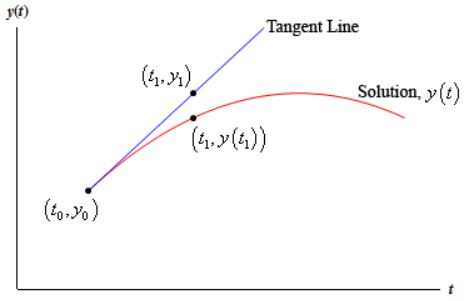
\includegraphics[scale=0.7]{Euler.JPG}
\end{figure}

\begin{itemize}
    \item If $t_1$ is close enough to $t_0$ then the point $y_1$ on the tangent line is a good
    approximation to the actual value of the solution $y(t_1)$ at $t_1$.
    
    $y_1$ is found by plugging $t_1$ into the equation for the tangent line:
    \begin{align*}
        y_1=y_0+f(t_0,y_0)(t_1-t_0)
    \end{align*}

    \item By proceeding in a similar manner, it could be repeated to get the values on the function.
    But only the value $t_0$ is known and $t_1, t_2, \dots$ is unknown. However, recall that $y_1$
    \textbf{is an approximation} to $t_1$ and, if it a good approximation, can be used as $t_1$ to
    obtain $t_2$:
    \begin{align*}
        y_2=y_1+f(t_1,y_1)(t_2-t_1)
    \end{align*}

    \item The process is then repeated:
    \begin{align*}
        y_3&=y_2+f(t_2,y_2)(t_3-t_2) \\
        y_4&=y_3+f(t_3,y_3)(t_4-t_3) \\
        \dots
    \end{align*}
\end{itemize}

\begin{tcolorbox}[colback=white]
The general equation of Euler's method is:
\begin{align*}
    y_{n+1}=y_n+f_n\; . \;(t_{n+1}-t_n)
\end{align*}
It is common to simplify the \textbf{step size} $t_{n+1}-t_n$ into $h$:
\begin{align*}
    y_{n+1}=y_n+h\:f_n
\end{align*}
\end{tcolorbox}

\textbf{Pseudocode}: 
\begin{lstlisting}[caption=Euler's Method: Pseudocode]
Start
    Define function f(x,y)

    Read values of initial condition(x0 and y0), number of steps (n) and calculation point (xn)
   
    Calculate step size (h) = (xn - x0)/n

    Set i=0

    Loop 
        yn = y0 + h *  f(x0 + i*h, y0)
      
        y0 = yn
      
        i = i + 1
    while i < n

    Display yn as result
Stop
\end{lstlisting}

\textbf{Python}: 
\begin{lstlisting}[caption=Euler's Method: Python code, language=Python, numbers=none]
"""
Euler's method.py:

The classical Euler's method to solve dy\dx = -6x
"""

import numpy as np
import matplotlib.pyplot as plt

x0 = 0
y0 = 1
h = 0.03
x_final = 1
N = round((x_final-x0)/h)

x = np.linspace(0,x_final,N) 
y = np.zeros(len(x)) 
y[0] = y0

for n in range(0,len(x) -1): 
    y[n+1] = (y[n] + h*(-6*y[n])) # Input the function equation

y_true = np.exp(-6*x) # Plot the true graph of function 'exp(-6x)'

""" Plotting program """

plt.plot(x,y,'b.-',x,y_true,'r-')
plt.legend(['Euler','True'])
plt.axis([0,2,0,9])
plt.grid(True)
plt.title("Solution of $y'=y , y(0)=1$")
plt.show()
\end{lstlisting}




%%%%%%%%%%%%%%%%%%%%%%%%%%%%%%%%%%%%%%%%%%%%%%%%%%%%%%%%%%%%%%%%%%%%%%%%%%%%%%%%%%%%%%%%%%%%%%%%%%%%%%%%%%
\subsubsection{Error analysis}

In Euler's method error analysis, the \textbf{local error} and \textbf{global error} is of concern.

The principal tool in the determination of truncation error is Taylor’s theorem, a key result in
calculus that provides a formula for the amount of error in using a truncated Taylor series to
represent the corresponding function.

\begin{center}
    \textit{Convention: Exact solution to ODE denoted by lower-case letter. Numerical approximations to ODE denoted by capital letter.}
\end{center}

\begin{tcolorbox}[breakable,colback=white]
    \textbf{Local truncation error}: A measure of accuracy over one step of a method for the numerical
    solution of ODEs.
\end{tcolorbox}

The \textit{local error} or \textit{error per step} is \textbf{proportional to the square of the
step size $h$}. 

\textbf{Derivation}: Taylor series for a function $x(t)$ defined as:
$$
    x(t+h)=x(t)+h\frac{dx}{dt}(t)+\frac{h^2}{2!}\frac{d^2x}{dt^2}(t)+\frac{h^3}{3!}\frac{d^3x}{dt^3}(t)+...
$$
\begin{center}
    or
\end{center}
$$
    x(t+h)=[x(t)]+h[x^\prime(t)]+\frac{h^2}{2!}[x^{\prime \prime}(t)]+\frac{h^3}{3!}[x^{\prime \prime \prime}(t)]+...
$$

Euler's method can be seen as using Taylor series \textbf{truncated after the second term} 
$h[x^{\prime}(t)]$ and given the value of $x(t)$ with its derivatives
of $x$ at $t$. 

It is possible to find the value of $x(t+h)$ for any given $h$ by choosing a small 
enough $h$ - it will provide a good approximation to the value of $x(t+h)$.
$$
    X(t+h) = x(t) + h\frac{dx}{dt}(t) = x(t) + hf(t,x)
$$
For example, applying it to points given the starting point $(t_0, x_0)$:
\begin{align*}
    X(t_1)&=X(t_0 + h) = x(t_0)+hf(t_0,x_0) \\
    X(t_2)&=X(t_1+h)=X(t_1)+hf(t_1,X_1) \\
    \dots
\end{align*}

Analysing Euler's method through application of Taylor series allows the accuracy of Euler's method
to be evaluated and to obtain more accurate methods. 

As stated earlier on the Taylor series:
$$
    x(t+h)=[x(t)]+h[f(t,x)]+\frac{h^2}{2!}[f^\prime (t,x)]
$$
Using the \textbf{order notation}, the equation is abbreviated to:
$$
    x(t+h)=[x(t)]+h[f(t,x)]+O(h^2)
$$
where $\frac{h^2}{2}f^\prime(t,x)=O(h^2)$

Combining it with Euler's method $X(t+h) = x(t) + hf(t,x)$:
$$
    X(t+h) = x(t+h) + O(h^2)
$$

The equation indicates that there is an \textbf{local truncation error} of order $h^2$ occurring in
each loop from $x(t)$ to $x(t+h)$. Some errors may cancel out as some cases it will be below true
value and some cases it will be above true value.

This is the reason Euler's method is known as a \textbf{first-order method}. The error, as it is 
dependent on the size of $h$, decreases as $h$ decreases i.e. halving the size of $h$ decreases
error by four times. 

\begin{tcolorbox}[breakable,colback=white,colframe=black,width=\dimexpr\textwidth+12mm\relax,enlarge left by=-6mm]
\textbf{Global truncation error}: The error in the value of $X(t_0 + a)$ obtained using a numerical
method to advance the required number of steps from a known value of $x(t_0)$
\end{tcolorbox}

The \textit{global error} or \textit{error at a given time} is proportional to the step size -
$O(h)$. 

\textbf{Derivation}:
\begin{itemize}
    \item Given a starting point $(x_0, y_0)$ and using Euler's method with a step size of $h$, a
    value of $X(t_0 + 4)$ will require $\frac{4}{h}$ steps. 
    \item Total error in $X(t_0 + 4)$ will be the sum of errors at each each step - $\frac{4}{h}$
    times the value of typical step error.
    \item Total error is order of $\left[\frac{4}{h}\right]O(h^2)$ which is $O(h)$ i.e. halving step
    size will halve the error in the solution.
\end{itemize}

%%%%%%%%%%%%%%%%%%%%%%%%%%%%%%%%%%%%%%%%%%%%%%%%%%%%%%%%%%%%%%%%%%%%%%%%%%%%%%%%%%%%%%%%%%%%%%%%%%%%%%%%%%
\subsubsection{Predictor-corrector method}

Improved Euler's method (Heun's method) is a second-order method and is composed of two equations:
\begin{enumerate}
    \item Predictor equation
    \item Corrector equation
\end{enumerate}

\textbf{Predictor equation}:

In Euler's method, the gradient \textbf{at the beginning of the interval} $[x_i, x_{i+1}]$:
$$
    y_i^{\prime}=f(x_i,y_i)
$$
is used to make a prediction of the value of $y_{i+1}$ at the end of the interval: 
$$
    y_{i+1}^p = y_i + hf(x_i,y_i)
$$
where $p$ as superscript indicates a prediction. \par 

\textbf{Corrector equation}:

Using the predicted value, an estimate of the gradient \textbf{at the end of the interval} is found:
$$
    y_{i+1}^{\prime} = f(x_{i+1},y_{i+1}^p)
$$

With the two gradient estimates at each end of the interval, an average can be found which is a
better estimate on the gradient over range $[x_i, x_{i+1}]$:
$$
    y_{av}^{\prime} = \frac{y_i^\prime + y_{i+1}^{\prime}}{2} = \frac{f(x_i,y_i)+f(x_{i+1},y_{i+1}^p)}{2}
$$

Using the average gradient and Euler's method, the corrector equation is defined:
$$
y_{i+1}=y_i+h\left(\frac{y_i^\prime + y_{i+1}^\prime}{2}\right)=y_i + h\left(\frac{f(x_i,y_i)+f(x_{i+1},y_{i+1}^p)}{2}\right)
$$

\begin{tcolorbox}[breakable,colback=white,colframe=black,width=\dimexpr\textwidth+12mm\relax,enlarge left by=-6mm]
\textbf{Improved Euler's method}:
\begin{itemize}
    \item Predictor equation:
    $$
        y_{i+1}^p = y_i + h[f(x_i, y_i)]
    $$
    \item Corrector equation:
    $$
        y_{i+1}=y_i +h\left[\frac{f(x_i,y_i)+f(x_{i+1},y_{i+1}^p)}{2}\right]
    $$
\end{itemize}
\end{tcolorbox}

\textbf{Example 1}: Solve the problem: $\frac{dx}{dt}=\frac{x^2}{t+1}$ given $x(0)=1$ with Improved
Euler's method.

\begin{enumerate}
    \item Predictor equation: 
    \begin{equation*}
        \begin{aligned}
            \hat{X}_1 &= x_0+h[f(t_0,x_0)] \\
            &= x_0 + h\left[\frac{x^2}{t+1}\right] \\
            &= 1 + 0.1\frac{1^2}{0+1} \\
            &= 1.100
        \end{aligned}
    \end{equation*}
    \item Corrector equation:
    \begin{equation*}
        \begin{aligned}
            X_1 &= x_0+\frac{1}{2}h[f(t_0,x_0)+f(t_1,\hat{X}_1)] \\
            &= x_0+\frac{1}{2}h\left[\frac{x_0^2}{t_0+1}+\frac{\hat{X}_1^2}{t_1 + 1}\right] \\
            &= 1.000 + \frac{1}{2}0.1\left[\frac{1^2}{0+1}+\frac{1.100^2}{0.100+1}\right] \\
            &= 1.105
        \end{aligned}
    \end{equation*}
\end{enumerate}

%%%%%%%%%%%%%%%%%%%%%%%%%%%%%%%%%%%%%%%%%%%%%%%%%%%%%%%%%%%%%%%%%%%%%%%%%%%%%%%%%%%%%%%%%%%%%%%%%%%%%%%%%%
\subsection{Runge-Kutta $2^{nd}$ order methods}

Runge-Kutta $2^{nd}$ Order method is a numerical technique used to solve a $1^{st}$ ordinary
differential equation of the form: 
$$
    \frac{dy}{dx}=f(x,y) \quad y(0)=y_0
$$

\textbf{Example 1}: Rewrite $\frac{dy}{dx}+2y=1.3e^{-x} \quad y(0)=5$ in the above format.
$$
    \frac{dy}{dx}=1.3e^{-x}-2y \quad y(0) = 5
$$

In the previous section with Euler's method, it was derived using information on the slope and the
derivative of $y$ at the given time step to derive the solution to the next time step. Runge-Kutta
methods are a \textbf{class of methods} that uses the same information at more than one point to
find the next time step. \par 

Euler's method was defined as:
$$
    y_{i+1} = y_i + f(x_i,y_i)h
$$
where: $x_0 = 0$, $y_0 = y(x_0)$ and $h=x_{i+1}-x_i$ \par 

Deriving Euler's method from Taylor series:
\begin{equation*}
    \begin{aligned}
        y_{i+1}&=y_i + \frac{dy}{dx}\rvert_{x_i,y_i} (x_{i+1}-x_i) + \frac{1}{2!}\frac{d^2 y}{dx^2}\rvert_{x_i,y_i} (x_{i+1}-x_i)^2 + \frac{1}{3!}\frac{d^3 y}{dx^3}\rvert_{x_i,y_i} (x_{i+1}-x_i)^3 + ... \\
        &= y_i + f(x_i,y_i)(x_{i+1}-x_i)+\frac{1}{2!}f^{\prime}(x_i,y_i)(x_{i+1}-x_i)^2+\frac{1}{3!}f^{\prime \prime}(x_i,y_i)(x_{i+1}-x_i)^3
    \end{aligned}
\end{equation*}

Notice the first two terms of the Taylor series: $y_{i+1}=y_i +f(x_i,y_i)h$ are Euler's method and
thus considered to be Runge-Kutta $1^{st}$ order method. The Runge-Kutta $2^{nd}$ order method will
include one more term of the Taylor series: 
$$
    y_{i+1} =  y_i + f(x_i,y_i)(x_{i+1}-x_i)+\frac{1}{2!}f^{\prime}(x_i,y_i)(x_{i+1}-x_i)^2
$$

However, there is certain difficulties in finding $f^{\prime}(x,y)$. Runge and Kutta simplified it
and wrote the general Runge-Kutta expression as: 

\begin{tcolorbox}[breakable,colback=white,colframe=black,width=\dimexpr\textwidth+12mm\relax,enlarge left by=-6mm]
$$
    y_{i+1}=y_i+h\phi(x_i,y_i,h)
$$
\end{tcolorbox}

where:
\begin{itemize}
    \item $\phi$ is the \textbf{increment function}: $\phi = a_1k_1+a_2k_2+...+a_nk_n$ 
    \item $a_i$ are constants
    \item $k_i$:
    \begin{equation*}
        \begin{aligned}
            k_1 &= f(x_i, \quad y_i) \\
            k_2 &= f(x_i+p_1h, \quad y_i+q_{11}k_1h) \\
            k_3 &= f(x_i + p_2h, \quad y_i + q_{21}k_1h + q_{22}k_2h)\\
            . \\
            . \\
            . \\
            k_n &= f(x_i + p_{n-1}h, \quad y_i + q_{n-1,1}k_1h + q_{n-1,2}k + 2h + ...+q_{n-1,n-1}k_{n-1}h)
        \end{aligned}
    \end{equation*}
\end{itemize}

\textbf{Example 2}: $2^{nd}$ order method is defined as:
$$
    y_{i+1}=y_i + (a_1k_1+a_2k_2)h
$$
where: 
\begin{itemize}
    \item $k_1 = f(x_i, \quad y_i)$
    \item $k_2 = f(x_i+p_1h, \quad y_i + q_{11}k_1h)$
\end{itemize}

%%%%%%%%%%%%%%%%%%%%%%%%%%%%%%%%%%%%%%%%%%%%%%%%%%%%%%%%%%%%%%%%%%%%%%%%%%%%%%%%%%%%%%%%%%%%%%%%%%%%%%%%%%
\subsubsection{Derivation of Second-order Runge-Kutta}

The value of $a$, $b$, $p$ and $q$ need to be found.
\begin{enumerate}
    \item Being with the equation: 
    $$
        y_{i+1}=y_i + (a_1k_1+a_2k_2)h
    $$
    where: 
    \begin{itemize}
        \item $k_1 = f(x_i, \quad y_i)$
        \item $k_2 = f(x_i+p_1h, \quad y_i + q_{11}k_1h)$
    \end{itemize}

    \item Use the Taylor expansion:
    $$
        y(x+h)=y(x)+hy^{\prime}(x)+\frac{h^2}{2!}y^{\prime \prime}(x)+\dots
    $$
    simplifies to:
    $$
        y_{i+1}=y_i + hf(x_i,y_i)+\frac{h^2}{2}f^{\prime}(x_i,y_i)+\dots
    $$

    \item Use partial differentiation:
    $$
        f^{\prime}(x,y) = \frac{\partial f(x,y)}{\partial x} + \frac{\partial f(x,y)}{\partial y} \frac{dy}{dx}
    $$

    \item Substitute into the Taylor expansion:
    $$
        y_{i+1}=y_i+hf(x_i,y_i)+\frac{h^2}{2}\left(\frac{\partial f}{\partial x} + \frac{\partial f}{\partial y}\frac{dy}{dx}\right) + \dots
    $$

    \item Recall Taylor expansion for function with two variables:
    $$
        F(x+h, \quad y+k) = F(x,y) + h\frac{\partial F}{\partial x} + k\frac{\partial F}{\partial y} + O(h^2,k^2)
    $$

    \item Consider $k_2 = f(x_i + ph, \quad y_i + qk_1h)$ and using Taylor expansion above:
    \begin{equation*}
        \begin{aligned}
            k_2 &= f(x_i + ph, \quad y_i+qk_1h) \\
            &= f(x_i, y_i) + ph\frac{\partial f}{\partial x} + qk_1h\frac{\partial f}{\partial y} + O(h^2)
        \end{aligned}
    \end{equation*}

    \item Substitute for $k_1$ and $k_2$ into $y_{i+1}=y_i + h(ak_1 + bk_2)$:
    \begin{equation*}
        \begin{aligned}
            y_{i+1} &= y_i hak_1 + hbk_2 \\
            &= y_i haf(x_i,y_i) + hb\left[f(x_i,y_i)+ph\frac{\partial f}{\partial x}+qf(x_i,y_i)h\frac{\partial f}{\partial y}+O(h^2)\right] \\
            &= y_i + (a+b)hf(x_i,y_i)+h^2\left(bp\frac{\partial f}{\partial x}+bq\frac{\partial f}{\partial y}f(x_i,y_i)\right) + O(h^3)
        \end{aligned}
    \end{equation*}

    \item Compare the two equations:
    $$
        y_{i+1}=y_i+hf(x_i,y_i)+\frac{h^2}{2}\left(\frac{\partial f}{\partial x} + \frac{\partial f}{\partial y}\frac{dy}{dx}\right) + \dots
    $$
    and
    $$
        y_{i+1}=y_i + (a+b)hf(x_i,y_i)+h^2\left(bp\frac{\partial f}{\partial x}+bq\frac{\partial f}{\partial y}f(x_i,y_i)\right) + O(h^3)
    $$
    
    \item Notice possible value:
    \begin{itemize}
        \item $a+b = 1$
        \item $bp=\frac{1}{2}$
        \item $bq=\frac{1}{2}$
    \end{itemize}
\end{enumerate}

\textbf{Example 3}: Heun's Method: Given $b=\frac{1}{2}$, $a=\frac{1}{2}$ and $p=q=1$:
$$
    y_{i+1}=y_i + h\left(\frac{1}{2}k_1 + \frac{1}{2}k_2\right)
$$
where the stages of Runge-Kutta $k_1=f(x_1, y_1)$ and $k_2=f(x_{i}+h, \quad y_{i}+k_1h)$ \par 

There are infinitely many types of Runge-Kutta methods due to the fact that each choice of $b$ gives
a new variation with roughly the same global error $O(h^2)$ with a few minor differences.

%%%%%%%%%%%%%%%%%%%%%%%%%%%%%%%%%%%%%%%%%%%%%%%%%%%%%%%%%%%%%%%%%%%%%%%%%%%%%%%%%%%%%%%%%%%%%%%%%%%%%%%%%%
\subsubsection{Improved Euler - Midpoint Method}

The Midpoint Method is another method that improved Euler's method that is based on using Euler's
method to estimate the gradient \textbf{at the midpoint of the interval} $[x_i,x_{i+1}]$. This gives
a better estimate of $y$ at the endpoint.

\begin{tcolorbox}[breakable,colback=white,colframe=black,width=\dimexpr\textwidth+12mm\relax,enlarge left by=-6mm]
\textbf{Midpoint method}: \par 
$$
    y_0=y(x_0)
$$
$$
    y_{i+\frac{1}{2}} = y_i + \frac{h}{2}f(x_i,y_i) 
$$
$$
    y_{i+1} = y_i + hf(x_{i+\frac{1}{2}},y_{i+\frac{1}{2}})
$$
\end{tcolorbox}

Operation:
$$
    k_1 = f(x_i,y_i)
$$
\begin{itemize}
    \item Using Euler's method to calculate gradient at $x_i$:
    $$
        k_2=f(x_i+\frac{1}{2}h, \quad y_i+\frac{1}{2}hk_1)
    $$
    \item Using Euler's method to calculate gradient at $x_i + \frac{h}{2}$:
    $$
        k_2 = f(x_i + \frac{1}{2}h, \quad y_i+\frac{1}{2}hk_1)
    $$
    \item Value used to calculate the endpoint:
    $$
        y_{i+1} = y_i + hk_2
    $$
\end{itemize}

\begin{figure} [h!]
    \centering
    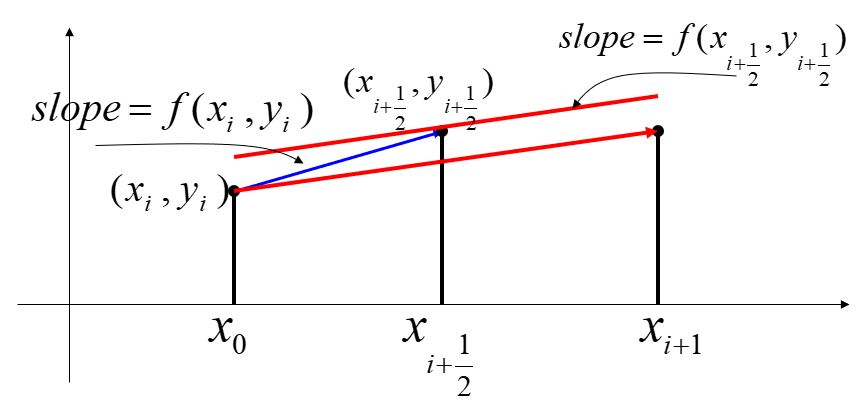
\includegraphics[scale=0.5]{Numerical.JPG}
    \caption{Graphical representation of Midpoint Method}
\end{figure}

\textbf{Local truncation error} of order $O(h^3)$ and \textbf{Global truncation error} of $O(h^2)$.

%%%%%%%%%%%%%%%%%%%%%%%%%%%%%%%%%%%%%%%%%%%%%%%%%%%%%%%%%%%%%%%%%%%%%%%%%%%%%%%%%%%%%%%%%%%%%%%%%%%%%%%%%%
\subsubsection{Higher-order Runge-Kutta methods}

There are infinitely many types of higher-order Runge-Kutta methods for example the classic $4^{th}$
order Runge-Kutta method:
\begin{equation*}
    \begin{aligned}
        k_1 &= f(x_i,\quad y_i) \\
        k_2 &= f(x_i+\frac{1}{2}h, \quad y_i+\frac{1}{2}k_1h) \\
        k_3 &= f(x_i+\frac{1}{2}h, \quad y_i+\frac{1}{2}k_2h \\
        k_4 &= f(x_i+h, \quad y_i+k_3h)
    \end{aligned}
\end{equation*}

%%%%%%%%%%%%%%%%%%%%%%%%%%%%%%%%%%%%%%%%%%%%%%%%%%%%%%%%%%%%%%%%%%%%%%%%%%%%%%%%%%%%%%%%%%%%%%%%%%%%%%%%%%
\section{Higher order ODE - Coupled $1^{st}$ order ODE}

The classes of second- and higher order differential equations with no analytical solution can be
solved by numerical means. Numerical solutions of second- and higher-order equations does not need
any new theory or technique.

%%%%%%%%%%%%%%%%%%%%%%%%%%%%%%%%%%%%%%%%%%%%%%%%%%%%%%%%%%%%%%%%%%%%%%%%%%%%%%%%%%%%%%%%%%%%%%%%%%%%%%%%%%
\subsection{Numerical solution of coupled first-order equations}

Given that first-order differential equations involve a single dependent variable and a single
independent variable, higher-order differential equations can be broken down into sets of coupled
first-order equations. Each equation involve the \textbf{same} independent variable but with
\textbf{more than one} dependent variable such as:
$$
    \frac{dx}{dt}=x-y^2+xt=f_1(t,x,y)
$$
$$
    \frac{dy}{dt}=2x^2+xy-t=f_2(t,x,y)
$$
The derivative of each dependent variables $x$ and $y$ depends on the independent variable $t$ and
the other dependent variable.

\begin{tcolorbox}[breakable,colback=white,colframe=black,width=\dimexpr\textwidth+12mm\relax,enlarge left by=-6mm]
    Original Euler's method: \par 
    $$
        X_{n+1}=X_n+hf(t_n,X_n)
    $$
    Euler's method on coupled first-order equations: \par 
    $$
        X_{n+1}=X_n+hf_1(t_n,X_n,Y_n)
    $$
    meaning value of $X_{n+1}$ depends on: $t_n$, $X_n$ and $Y_n$.
\end{tcolorbox}

\textbf{Example 1}: Using Euler's method with time step $h=0.1$, find the value of $X(1.2)$
satisfying the following initial value problem:
$$
    \frac{dx}{dt}=x-y^2+xt, \quad x(1)=0.5
$$
$$
    \frac{dy}{dt}=2x^2+xy-t, \quad y(1)=1.2
$$
\begin{enumerate}
    \item Denote right-hand side of two equations as $f_1(t,x,y)$ and $f_2(t,x,y)$, first step is:
    $$
        f_1(t,x,y)=x-y^2+xt \quad \text{and} \quad f_2(t,x,y)=2x^2+xy-t
    $$

    \item Note imposed initial equations $x_0=0.5$ and $y_0=1.2$:
    \begin{align*}
        X_1&=x_0+hf_1(t_0,x_0,y_0) & Y_1&=y_0+hf_2(t_0,x_0,y_0) \\
        &= 0.5 + 0.1f_1(1,0.5,1.2) & &=1.2+0.1f_2(1,0.5,1.2) \\
        &= 0.4560 & &= 1.2100
    \end{align*}

    \item Second step is (final step since $1+2(0.1) = 1.2$):
    \begin{align*}
        X_2&=X_1+hf_1(t_1,x_1,y_1) & Y_2&=Y_1+hf_2(t_1,x_1,y_1) \\
        &= 0.4560 + 0.1f_1(1.1,0.4560,1.2100) & &=1.2100+0.1f_2(1.1,0.4560,1.2100) \\
        &= \underline{0.4054} & &= 1.1968
    \end{align*}
\end{enumerate}

\textbf{Example 2}: Find the value of $X(1.2)$ satisfying the initial-value problem:
$$
    \frac{dx}{dt}=x-y^2+xt \quad x(1)=0.5 
$$
$$
    \frac{dy}{dt}=2x^2+xy-t \quad y(1)=1.2
$$
using the second-order predictor-corrector method with time step $h=0.1$.

\begin{itemize}
    \item First step:
    \begin{enumerate}
        \item Find the predictor equation, noting the initial conditions:
        \begin{align*}
            \hat{X}_1&=x_0+hf_1(t_0,x_0,y_0) & \hat{Y}_1&=y_0+hf_2(t_0,x_0,y_0) \\
            &= 0.4560 & &= 1.2100
        \end{align*}
        \item Find the corrector equation, using the values obtained from the predictor:
        \begin{align*}
            \hat{X}_1&=x_0+\frac{1}{2}h[f_1(t_0,x_0,y_0)+f_1(t_1,\hat{X}_1,\hat{Y}_1)] \\
            &= 0.5 + 0.05[f_1(1,0.5,1.2)+f_1(1.1,0.456,1.21)] \\
            &= 0.4527
        \end{align*}
        \begin{align*}
            \hat{Y}_1&=y_0+\frac{1}{2}h[f_2(t_0,x_0,y_0)+f_2(t_1,\hat{X}_1,\hat{Y}_1)] \\
            &= 1.2+0.05[f_2(1,0.5,1.2)+f_2(1.1,0.456,1.21)] \\
            &= 1.1984
        \end{align*}
    \end{enumerate} 
    \item Second step:
    \begin{enumerate}
        \item Find the predictor equation, noting the initial conditions:
        \begin{align*}
            \hat{X}_2&=x_1+hf_1(t_1,x_1,y_1) & \hat{Y}_2&=y_1+hf_2(t_1,x_1,y_1) \\
            &= 0.4042 & &= 1.1836
        \end{align*}
        \item Find the corrector equation, using the values obtained from the predictor:
        \begin{align*}
            \hat{X}_2&=X_1+\frac{1}{2}h[f_1(t_1,X_1,Y_1)+f_1(t_2,\hat{X}_2,\hat{Y}_2)] \\
            &= 0.4527 + 0.05[f_1(1.1,0.4527,1.1984)+f_1(1.2,0.4042,1.1836)] \\
            &= \underline{0.4028}
        \end{align*}
        \begin{align*}
            \hat{Y}_2&=Y_1+\frac{1}{2}h[f_2(t_1,Y_1,Y_1)+f_2(t_2,\hat{X}_2,\hat{Y}_2)] \\
            &= 1.1984+0.05[f_2(1.1,0.4527,1.1984)+f_2(1.2,0.4042,1.1836)] \\
            &= 1.1713
        \end{align*}
    \end{enumerate} 
\end{itemize}

%%%%%%%%%%%%%%%%%%%%%%%%%%%%%%%%%%%%%%%%%%%%%%%%%%%%%%%%%%%%%%%%%%%%%%%%%%%%%%%%%%%%%%%%%%%%%%%%%%%%%%%%%%
\section{Finite Differences for ODEs (Boundary value problems)}

First-order ODEs have only one boundary condition treated as an initial condition. With second- and
higher-order, there are more than one boundary conditions such as:
$$
    y^{\prime \prime} - 2y^{\prime} + 3y = \sin(x) \quad \text{with} \quad y(0)=0 \text{ and } y(1)=0
$$

Boundary value problems do not always have solutions and prior analysis would usually be required to
determine the presence of a solution. For Year 2 Numerical Methods, boundary value problems are
assumed to have a solution. \par 

The previous approach will not work as the boundary conditions provided do not provide enough
information to approximate it using a system of first-order equations and there is no guarantee the
iteration would lead to the solution as given. \par

%%%%%%%%%%%%%%%%%%%%%%%%%%%%%%%%%%%%%%%%%%%%%%%%%%%%%%%%%%%%%%%%%%%%%%%%%%%%%%%%%%%%%%%%%%%%%%%%%%%%%%%%%%
\subsection{Central difference method}

One method of solving boundary value problems is based in by breaking up the interval in
question.\par 

An important concept is \textbf{Central Difference}: 
$$
    \delta y(x_i)=y\left(x_i + \frac{h}{2}\right)-y\left(x_i-\frac{h}{2}\right)
$$
Also note the approximation of derivative $\frac{dy}{dx}|_{x=x_i}$:
$$
    \frac{1}{h}\delta y(x_i) = \frac{y\left(x_i + \frac{h}{2}\right)-y\left(x_i-\frac{h}{2}\right)}{h} \approx \frac{dy}{dx}|_{x=x_i}
$$

Derivation:
\begin{enumerate}
    \item Define first central difference:
    $$
        \delta y(x_i)=y\left(x_i + \frac{h}{2}\right)-y\left(x_i-\frac{h}{2}\right)
    $$

    \item Define second central difference $\delta^2y(x_i)$:
    \begin{align*}
        \delta^2y(x_i)&=\delta[\delta y(x_i)]\\
        &= \delta y\left(x_i + \frac{h}{2}\right) - \delta y \left(x_i - \frac{h}{2}\right) \\
        &= \left\{y\left[\left(x_i + \frac{h}{2}+\frac{h}{2}\right)\right]-\left[\left(x_i+\frac{h}{2}\right)-\frac{h}{2}\right]\right\} - \left\{y\left[\left(x_i - \frac{h}{2}\right)+\frac{h}{2}\right]-y\left[\left(x_i - \frac{h}{2}\right)-\frac{h}{2}\right]\right\} \\
        &= y(x_i + h) - 2y(x_i) + y(x_i - h)
    \end{align*}

    \item Second derivative $y^{\prime \prime}$ is defined as:
    $$
        \frac{1}{h^2} \delta^2 y(x_i) \approx \frac{d^2y}{dx^2}|_{x=x_i}
    $$
    
    \item Approximate of first derivative defined as:
    \begin{align*}
        \frac{1}{2h}\Delta y(x_i) &= \frac{y(x_i+h)-y(x_i - h)}{2h} \\
        &= \frac{y(x_{i+1})-y(x_{i-1})}{2h} \\
        &= \frac{dy}{dx} |_{x=x_i}
    \end{align*}
    
    \item Let $u_i \approx  y(x_i)$
    \begin{tcolorbox}[breakable,colback=white,colframe=black,width=\dimexpr\textwidth+12mm\relax,enlarge left by=-6mm]
        \textbf{Central difference method}: 
    \begin{align*}
        \frac{dy}{dx}|_{x=x_i} \approx \frac{u_{i+1}-u_{i-1}}{2h} \quad \text{and} \quad \frac{d^2 y}{dx^2}|_{x=x_i} \approx \frac{u_{i+1}-2u_i+u_{i-1}}{h^2}
    \end{align*}
    \end{tcolorbox}
\end{enumerate}

\textbf{Example 1}: Solve the given model convection-diffusion equation:
$$
    y^{\prime \prime} - 20y^{\prime}=-1 \quad \text{where} \quad y(0)=1 \text{ and } y(1)=0
$$
\begin{enumerate}
    \item Divide interval of interest $[0,1]$ into five segments, forming step size $h=0.2$ into the
    following: $x_0=0$, $x_1=0.2$, $x_2=0.4$, $x_3=0.6$, $x_4=0.8$ and $x_5=1.0$.

    \item Estimate derivatives using formulae:
    $$
        \frac{u_{i+1}-2u_i+u_{i-1}}{h^2} - 20\left(\frac{u_{i+1}-u_{i-1}}{2h}\right)=-1
    $$
    Rearrange into:
    $$
        \left(\frac{10}{h}+\frac{1}{h^2}\right)u_{i-1} - \frac{2}{h^2}u_i + \left(-\frac{10}{h}+\frac{1}{h^2}\right)u_{i+1} = -1
    $$  
    $$
        au_{i-1} + bu_i + cu_{i+1} = -1
    $$

    \item For each $i$, there is an equation defined by $u_{i-1}$, $u_i$ and $u_{i+1}$:
    \begin{align*}
        i &= 1: \quad au_0+bu_1+cu_2 = -1 \\
        i &= 2: \quad au_1+bu_2+cu_2 = -1 \\
        i &= 3: \quad au_2+bu_3+cu_4 = -1 \\
        i &= 4: \quad au_3+bu_4+cu_5 = -1 
    \end{align*}
    where $u_0$ and $u_5$ are known boundary values.

    \item Express in matrix form:
    $$
    \begin{bmatrix} 
        b&c&0&0 \\
        a&b&c&0 \\
        0&a&b&c \\
        0&0&a&b
    \end{bmatrix} 
    *
    \begin{bmatrix}
        u_1 \\
        u_2 \\
        u_3 \\
        u_4
    \end{bmatrix}
    =
    \begin{bmatrix}
        -1-au_0 \\
        -1 \\
        -1 \\
        -1 - cu_5
    \end{bmatrix}
    $$

    \item Use Gaussian elimination to obtain the solutions:
    \begin{align*}
        u_1 \approx 0.9928 \quad u_2 \approx 1.0544 \quad u_3 \approx 0.9095 \quad u_4 \approx 1.3843
    \end{align*}
\end{enumerate}

%%%%%%%%%%%%%%%%%%%%%%%%%%%%%%%%%%%%%%%%%%%%%%%%%%%%%%%%%%%%%%%%%%%%%%%%%%%%%%%%%%%%%%%%%%%%%%%%%%%%%%%%%%
\section{Partial Differential Equations}

The method of finite differences extends to solution of partial differential equations. Many
solutions exists for many types of partial differentials. Two examples of Partial Differential
Equations and a method to solve are given.

%%%%%%%%%%%%%%%%%%%%%%%%%%%%%%%%%%%%%%%%%%%%%%%%%%%%%%%%%%%%%%%%%%%%%%%%%%%%%%%%%%%%%%%%%%%%%%%%%%%%%%%%%%
\subsection{Heat/Diffusion equation}

\begin{tcolorbox}[breakable,colback=white,colframe=black,width=\dimexpr\textwidth+12mm\relax,enlarge left by=-6mm]
General form of the Heat/Diffusion equation:
$$
    \frac{\partial y}{\partial t} = \frac{\partial ^2y}{\partial x^2} \quad 0<x<1 \text{ and } t>0
$$
with boundary conditions $y(0,t)=y(1,t)=0$ and initial condition $y(x,0)=y_0(x)$
\end{tcolorbox}

The heat/diffusion equation describes the temperature distribution in a thin metal rod of unit
length with insulated sides and both ends kept at $0K$. \par 

At time $t=0$, distribution is $y_0(x)$ and solution to the partial differential describes evolution
in time. It can also describe other diffusive processes such as pollutant gas in a pipe or random
walk. \par 

Finite differences (central difference) will be used for both derivatives:
\begin{enumerate}
    \item Divide the spatial interval into $N$ segments of equal length $h=\frac{1}{N}$:
    $$
        x_0=0;x_1=h;x_2=2h;\dots;x_N=Nh=1
    $$

    \item Divide the time domain into equal segments of length $k$:
    $$
        t_0=0;t_1=k;t_2=2k
    $$
    where there is no clear end, the process is repeated as far as required

    \item Let $U_j^m$ be value $y(x_j,t_m)$ where the initial condition gives the values of $y$ at $t=0$:
    $$
        U_j^0=y(x_j,t_0)=y(x_j,0) = y_0(x_j) \quad \text{for } j=0,1,2,\dots, N
    $$

    \item The boundary conditions gives values for $j=0$ corresponding to $x=$ and for $j=n$
    corresponding to $x=1$:
    $$
        U_j^m=y(x_j,t_m) \rightarrow y(0,t_m) = U_0^m = 0 \quad \text{and} \quad y(1,t_m)=U_N^m = 0
    $$
    where $\forall m \geq 0$

    \item Recall function of two variables to deal with spatial derivative:
    $$
        \frac{\partial^2y(x,t)}{\partial x^2} \approx \frac{y(x+h,t)-2y(x,t)+y(x-h,t)}{h^2}
    $$
    where $t$ remains constant and $x$ varies by $h$ in both directions \par 

    \textbf{Working example 1}: Given $t=t_m$ and $x=x_j$ which leads to $x\pm h = x_{j\pm 1}$
    \begin{align*}
        \frac{\partial^2 y(x_j,t_m)}{\partial x^2} &\approx \frac{y(x_{j+1},t_m) - 2y(x_j,t_m)+y(x_{j-1},t_m)}{h^2} \\
        &\approx \frac{U_{j+1}^m - 2U_j^m + U_{j-1}^m}{h^2} \quad j=1,2,\dots,N-1
    \end{align*}

    \item For the time derivative, use a \textbf{"forward difference"}:
    $$
        \frac{\partial y(x,t)}{\partial t} \approx \frac{y(x,t+k)-y(x,t)}{k}
    $$
    A forward difference must be used as there cannot be $t=-1$ \par 

    \textbf{Working example 2}: Given $t=t_m$ and $x=x_j$ which leads to $t+k = t_{m+1}$
    \begin{align*}
        \frac{\partial y(x_j,t_m)}{\partial t} &\approx \frac{y(x_j,t_{m+1})-y(x_j,t_m)}{k} \\
        &\approx \frac{U_j^{m+1}-U_j^m}{k} \quad m=0,1,2,3\dots
    \end{align*}

    \item Set two derivatives equal:
    $$
        \frac{U_{j+1}^m - 2U_j^m + U_{j-1}^m}{h^2} = \frac{U_j^{m+1}-U_j^m}{k}
    $$
    Let $v=\frac{k}{h^2}$
    $$
        v\left(U_{j+1}^m - 2U_j^m + U_{j-1}^m\right) = U_j^{m+1} - U_j^m
    $$

    \item Express in terms of $U_j^{m+1}$:
    \begin{align*}
        U_j^{m+1} &= U_j^m + v\left(U_{j+1}^m - 2U_j^m + U_{j-1}^m\right) \\
        &= vU_{j-1}^m + (1-2v)U_j^m + vU_{j+1}^m
    \end{align*}
\end{enumerate}

%%%%%%%%%%%%%%%%%%%%%%%%%%%%%%%%%%%%%%%%%%%%%%%%%%%%%%%%%%%%%%%%%%%%%%%%%%%%%%%%%%%%%%%%%%%%%%%%%%%%%%%%%%
\subsection{Laplace/Poisson equation}

Laplace's second-order equation is widely used in physics since its solutions occur in fields such
as electrical, magnetic and gravitational. Poisson's equation is a generalisation of Laplace's
equation that is widely used in theoretical physics e.g. the solution to the potential field caused
by a given electrical charge or mass density distribution. \par 

\begin{tcolorbox}[breakable,colback=white,colframe=black,width=\dimexpr\textwidth+12mm\relax,enlarge left by=-6mm]
\textbf{Poisson' equation}: 
$$
    \frac{\partial^2 u}{\partial x^2} + \frac{\partial^2 u}{\partial y^2} = g(x,y)
$$
where Laplace's equation is given when $g=0$ 
\end{tcolorbox}

The central difference is used to approximate the two derivatives:
\begin{align*}
    \frac{\partial ^2 u(x,y)}{\partial x^2} &\approx \frac{u(x+h,y)-2u(x,y)+u(x-h,y)}{h^2} \\
    \frac{\partial^2u(x_i,y_j)}{\partial x^2} &\approx \frac{u(x_{i+1},y_j)-2u(x_i,y_j)+u(x_{i-1},y_j)}{h^2} \\
    &= \frac{U_{i+1}^j - 2U_i^j + U_{i-1}^j}{h^2}
\end{align*}
and
\begin{align*}
    \frac{\partial ^2 u(x,y)}{\partial y^2} &\approx \frac{u(x,y+h)-2u(x,y)+u(x,y-h)}{h^2} \\
    \frac{\partial^2u(x_i,y_j)}{\partial y^2} &\approx \frac{u(x_{i},y_{j+1})-2u(x_i,y_j)+u(x_{i},y_{j-1})}{h^2} \\
    &= \frac{U_{i}^{j+1} - 2U_i^j + U_{i}^{j-1}}{h^2}
\end{align*}

As mentioned earlier, Laplace's equation is found when the sum of the two derivatives is set to 0.
An approximation of Laplace's equation is found when using the central difference of the two
derivatives:
\begin{align*}
    \frac{U_{i+1}^j - 2U_i^j + U_{i-1}^j}{h^2} + \frac{U_i^{j+1}-2U_i^j + U_i^{j-1}}{h^2} = 0 
\end{align*}
Simplifies to:
\begin{align*}
    U_{i+1}^j + U_{i-1}^j + U_i^{j+1} + U_i^{j-1} - 4U_i^{j-1} - 4U_i^j = 0
\end{align*}

\textbf{Worked Example 1}: The simplest case of Laplace's equation is on a rectangle: $0\leq x\leq
a$ and $0\leq y \leq b$ divided into $(n-1)x(m-1)$ squares with side length $h$. This means: 
\begin{itemize}
    \item $a=nh$ and $b=mh$
    \item $i=1\dots n$ and $j=1\dots m$ 
\end{itemize}

\begin{figure} [h!]
    \centering
    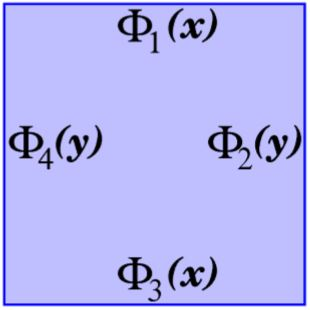
\includegraphics[scale=0.4]{Square.JPG}
    \caption{Graphical representation of the locations of $\phi$}
\end{figure}

The solution requires knowledge of $u$ on the shape boundaries (Boundary Conditions):
\begin{itemize}
    \item $\phi_1(x)$ where $y=b$ giving the values $U_i^m$ for $i=1\dots n$
    \item $\phi_2(x)$ where $x=a$ giving the values $U_n^j$ for $i=1\dots m$
    \item $\phi_3(x)$ where $y=0$ giving the values $U_i^1$ for $i=1\dots n$
    \item $\phi_4(x)$ where $y=0$ giving the values $U_1^j$ for $i=1\dots m$
\end{itemize}

\begin{figure} [h!]
    \centering
    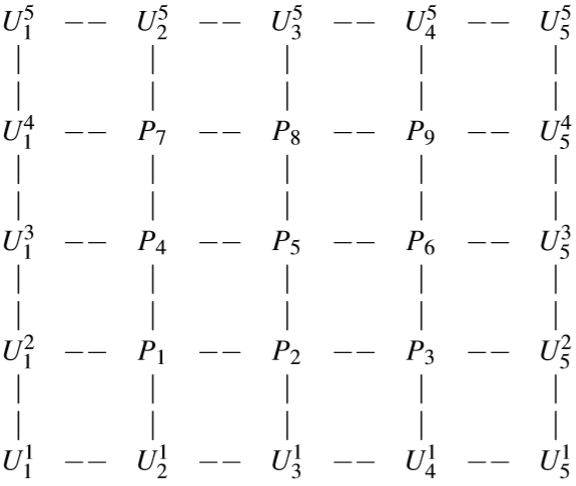
\includegraphics[scale=0.4]{Square_broken.JPG}
    \caption{Square broken down into points with $U$ known and $P$ unknown}
\end{figure}

The values on the edges $U_i^j$ are known from Boundary Conditions, only the interior points $P_1
\dots P_9$ are unknown. The approximation of Laplace's equation is defined: 
$$
    U_{i+1}^j + U_{i-1}^j + U_i^{j+1} + U_i^{j-1} - 4U_i^j = 0
$$
which is a relationship that involves five points: 
\begin{itemize}
    \item Center at $x_i,y_i$
    \item Above at $U_i^{j+1}$
    \item Below at $U_i^{j-1}$
    \item Right at $U_{i+1}^j$
    \item Left at $U_{i-1}^j$
\end{itemize} 

This relationship can be applied where every unknown interior point is taken as the centre. For example:
\begin{align*}
    \text{at } P_1: U_1^2+U_2^1+P_2+P_4-4P_1 = 0 \\
    \text{at } P_2: P_1+U_3^1+P_3+P_5-4P_2 = 0 \\
    \text{at } P_3: P_2+U_4^1+U_5^2+P_6-4P_3 = 0 
\end{align*}

The equations can be rewritten in matrix form to be solved as usual:
$$
\begin{bmatrix}
    -4&1&0&1&0&0&0&0&0 \\
    0&-4&1&0&1&0&0&0&0 \\
    0&1&-4&0&0&1&0&0&0 \\
    1&0&0&-4&1&0&1&0&0 \\
    0&1&0&1&-4&1&0&1&0 \\
    0&0&1&0&1&-4&0&0&1 \\
    0&0&0&1&0&0&-4&1&0 \\
    0&0&0&0&1&0&1&-4&1 \\
    0&0&0&0&0&1&0&1&-4
\end{bmatrix} 
*
\begin{bmatrix}
    P_1 \\
    P_2 \\
    P_3 \\
    P_4 \\
    P_5 \\
    P_6 \\
    P_7 \\
    P_8 \\
    P_9
\end{bmatrix}
$$

As solving via matrix is a computationally expensive task, an alternative is the \textbf{Relaxation method}.

%%%%%%%%%%%%%%%%%%%%%%%%%%%%%%%%%%%%%%%%%%%%%%%%%%%%%%%%%%%%%%%%%%%%%%%%%%%%%%%%%%%%%%%%%%%%%%%%%%%%%%%%%%
\subsection{Relaxation method}

The relaxation method is based on the \textbf{continuity of solutions}.
\begin{tcolorbox}[breakable,colback=white,colframe=black,width=\dimexpr\textwidth+12mm\relax,enlarge left by=-6mm]
\textbf{Continuity of solutions}: \par 
Able to take each point as the average of its four nearest neighbours: 
    \begin{align*}
        U_j^i &= \frac{(U_{i+1}^j + U_{i-1}^j + U_i^{j+1} + U_i^{j-1})}{4} \\
        &= \frac{U_{i+1}^j + U_{i-1}^j + U_i^{j+1} + U_i^{j-1} - 4U_i^j}{4} = 0
    \end{align*}
\end{tcolorbox}

\begin{enumerate}
    \item Set all points inside grid to an initial value $k$ - average of values of known boundary points
    \item For each interior point, calculate:
    $$
        \left(U_i^j\right)_{new} = \left(U_i^j\right)_{old} + r_i^j
    $$
    where the \textbf{residual} $r_{ij}$ is given by:
    $$
        r_i^j = \frac{U_{i+1}^j + U_{i-1}^j + U_i^{j+1} + U_i^{j-1} - 4U_i^j}{4}
    $$
    \begin{itemize}
        \item The residual vanishes as the averages are recalculated repeatedly
        \item Set a desired accuracy $\epsilon > 0$ and stop when $|r_i^j|<\epsilon$ at every
        interior point
    \end{itemize}
\end{enumerate}

Poisson equation can be easily incorporated into the relaxation methods by taking $g(x_i,y_j)=g_i^j$
for example:
$$
r_i^j = \frac{U_{i+1}^j + U_{i-1}^j + U_i^{j+1} + U_i^{j-1} - 4U_i^j - h^2g_i^j}{4}
$$

%%%%%%%%%%%%%%%%%%%%%%%%%%%%%%%%%%%%%%%%%%%%%%%%%%%%%%%%%%%%%%%%%%%%%%%%%%%%%%%%%%%%%%%%%%%%%%%%%%%%%%%%%%
\section{Summary}
%%%%%%%%%%%%%%%%%%%%%%%%%%%%%%%%%%%%%%%%%%%%%%%%%%%%%%%%%%%%%%%%%%%%%%%%%%%%%%%%%%%%%%%%%%%%%%%%%%%%%%%%%%
\subsection{Numerical methods for initial-value problems}

MIT Numerical

%%%%%%%%%%%%%%%%%%%%%%%%%%%%%%%%%%%%%%%%%%%%%%%%%%%%%%%%%%%%%%%%%%%%%%%%%%%%%%%%%%%%%%%%%%%%%%%%%%%%%%%%%%
\section{Introduction}
%%%%%%%%%%%%%%%%%%%%%%%%%%%%%%%%%%%%%%%%%%%%%%%%%%%%%%%%%%%%%%%%%%%%%%%%%%%%%%%%%%%%%%%%%%%%%%%%%%%%%%%%%%
\subsection{Trapezoid Rule}

Not every integral has an exact solution, the solution will have to be approximated using a
numerical technique such as the Trapezoid Rule. \par 

Given the integral of $f(x)$ over interval $[a,b]$, divide the interval into $n$ segments of equal
length defined as $h=\frac{b-a}{n}$.

\begin{figure} [h!]
    \centering
    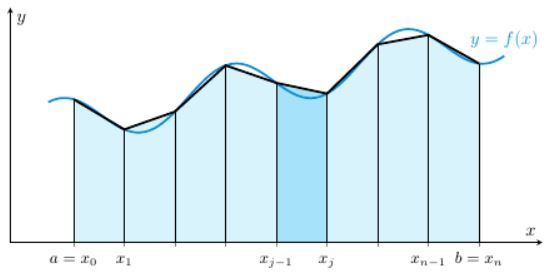
\includegraphics[scale=0.6]{Trapezoid.JPG}
    \caption{Graphical representation of the Trapezoid Rule}
\end{figure}

From the picture:
\begin{itemize}
    \item Set $a=x_0$ and $b=x_n$
    \item $n$ intervals are $[x_i,x_{i+1}]$ for $i=0...n-1$
\end{itemize}

Since the area under the curve $f(x)$ is divided into segments, the area under the curve
(integration):
$$
\int_{x_i}^{x_{i+1}} f(x) \text{ dx}
$$
is the approximated to the average of the area of left trapezoid $f(x_i)$ and right trapezoid
$f(x_{i+1})$:
$$
\int_{x_i}^{x_{i+1}} f(x) \text{ dx} \approx \frac{1}{2}h[f(x_i)+f(x_{i+1})]
$$

\begin{tcolorbox}[breakable,colback=white,colframe=black,width=\dimexpr\textwidth+12mm\relax,enlarge left by=-6mm]
    The general case for the Trapezoid Rule is defined as:
    $$
    \int_a^b f(x)\text{ dx} \approx \left(\frac{b-a}{2n}\right)\left[f(x_0)+2\left(\sum_{i=1}^{n-1}f(x_i)\right)+f(x_n)\right]
    $$
\end{tcolorbox}

\textbf{Example 1}: Given $n=3$, $a=x_0$ and $b=x_3$, the general case becomes: 
$$
\frac{1}{2}f\left[f(x_0)+f(x_1)\right]+\frac{1}{2}h\left[f(x_1)+f(x_2)\right]+\frac{1}{2}f\left[f(x_2)+f(x_3)\right]
$$

%%%%%%%%%%%%%%%%%%%%%%%%%%%%%%%%%%%%%%%%%%%%%%%%%%%%%%%%%%%%%%%%%%%%%%%%%%%%%%%%%%%%%%%%%%%%%%%%%%%%%%%%%%
\section{Change of Variables}
%%%%%%%%%%%%%%%%%%%%%%%%%%%%%%%%%%%%%%%%%%%%%%%%%%%%%%%%%%%%%%%%%%%%%%%%%%%%%%%%%%%%%%%%%%%%%%%%%%%%%%%%%%
\subsection{One function of two random variables}

Given two random variables $X$ and $Y$ characterized by the joint PDF $f_{X,Y}(x, y)$ and a function $g(x, y)$, a new random
variable $Z$ is formed as $Z = g(X,Y)$. The PDF of $Z$ denoted $f_Z(z)$ can be calculated.

This situation occurs commonly in practical applications such as a receiver output signal $Z$ which
consists of the desired signal $X$ that is buried in the noise $Y$ thus leading to: $Z = X+Y$

\begin{tcolorbox}[breakable,colback=white]
\textbf{If two random variables are independent then the density of their sum is equal to the convolution of their density function.}
\begin{align*}
    f_Z = f_X \otimes f_Y
\end{align*}
\begin{align*}
    f_Z(z) = \int_{x=-\infty}^{x=+\infty} f_{XY}(x,z-x)\: dx = \int_{y=-\infty}^{y=+\infty} f_{XY}(z-y,y)\: dy 
\end{align*}
If $X$ and $Y$ are independent then $f_{XY}(x,y)=f_X(x)f_Y(y)$:
\begin{align*}
    f_Z(z)=\int_{y=-\infty}^{y=+\infty} f_X(z-y)f_Y(y)\:dy = \int_{x=-\infty}^{x=+\infty} f_X(x)f_Y(z-x)\:dx
\end{align*}
\end{tcolorbox}

%%%%%%%%%%%%%%%%%%%%%%%%%%%%%%%%%%%%%%%%%%%%%%%%%%%%%%%%%%%%%%%%%%%%%%%%%%%%%%%%%%%%%%%%%%%%%%%%%%%%%%%%%%
\subsection{Two functions of two random variables}



%%%%%%%%%%%%%%%%%%%%%%%%%%%%%%%%%%%%%%%%%%%%%%%%%%%%%%%%%%%%%%%%%%%%%%%%%%%%%%%%%%%%%%%%%%%%%%%%%%%%%%%%%%
\end{document}